\documentclass[10pt,letterpaper]{article}
\usepackage[margin=0.72in]{geometry}
\usepackage[T1]{fontenc}
\usepackage{lmodern,amsmath,amssymb,booktabs,graphicx,float,array,longtable,url}
\usepackage[font=small,labelfont=bf]{caption}
\renewcommand{\thetable}{S\arabic{table}}
\renewcommand{\thefigure}{S\arabic{figure}}
\setlength{\parindent}{0pt}
\setlength{\parskip}{5pt}
\setlength{\tabcolsep}{4pt}
\raggedbottom
\begin{document}
\begin{center}{\Large\bfseries Supplementary Information}\\[5pt]

Paired Fault Assessment of a Fly-Connectome Spiking Controller
\\[5pt]Shuchao Gao, Waseda University\\
Assessment v9: matched source, data and protocol\end{center}
This document separates the independent core test, a prespecified angle stress
test, development, and historical audits. Every new table is reconstructed from
saved raw records and frozen registrations. Historical observations are retained
with their original limitations; they are not silently relabeled as new experiments.
\section{Protocol, software and calibration}
The current task is \texttt{task-v9.1-causal-exact-events}. The main Methods and
\path{paper/PROTOCOL_v9.md} define the sampled plant, common-random-number coupling,
first-passage task outcome and resource estimands. All test parameters were frozen
before outcomes. The neural substrate uses released FlyWire v783 tables and Shiu
parameters; the original publication used v630. The synthetic visual/body coupling
is not validated fly behavior. Functional row deletions are not physical bit faults.
Between spikes the voltage and voltage-valued synaptic drive obey
\[
\dot v_i=(v_0-v_i+g_i)/(20\,\mathrm{ms}),\qquad
\dot g_i=-g_i/(5\,\mathrm{ms}).
\]
Recurrent events add signed contact counts times 0.275\,mV to $g_i$ after
1.8\,ms. At threshold $-45$\,mV, reset sets $v_i$ to $v_0=-52$\,mV and
$g_i$ to zero; both equations pause during 2.2\,ms refractoriness. Sensory
cells retain this refractoriness, a variant of upstream stimulation. External
events add 68.75\,mV to voltage; all non-sensory external rates are zero.
Initial neural states, monitors and unmodified recurrent weights are restored
before each episode. A separate tiny actual Brian2 test verifies this reset,
including reapplying external weights, without loading a full connectome.

\begin{table}[H]
\centering\small
\caption{Fixed physical settings. No hardware power or area is inferred.}
\begin{tabular}{lr}
\toprule
Parameter & Value\\
\midrule
Neural / feedback step & 0.1 / 20 ms\\
Cue / task horizon & 100 / 1000 ms\\
Pursuer speed / initial separation & 0.3 m/s / 0.25 m\\
Contact / looming radius & 0.05 / 0.05 m\\
Walk / burst speed & 0.05 / 0.35 m/s\\
Burst delay / duration & 250 / 450 ms\\
Common turn limit / heading cap & 600 deg/s / $\pm100$ deg\\
RF seed / inactive pool seed & 20260201 / 0\\
\bottomrule
\end{tabular}
\end{table}

Independent input streams use SeedSequence [20261022, seed, frame, 1]; deletion uses [20261022, seed, 2]. The former supplies float32 cell/time uniforms and the latter float64 row uniforms. Both doses reuse the same row variates. Actual realized contact mass and sign composition are saved, not forced to equal their expectations. The input map saves pool/sensory/command identities and RF parameters. Exact source and table hashes are bound by the JSON registrations.

\begin{table}[H]
\centering\small
\caption{Fitted direction decoder coefficients, raw five-frame Hz features. Intercept is 0.026677472.}
\begin{tabular}{lrrr}
\toprule
FlyWire ID & Type & Side & $\beta_i$\\
\midrule
720575940622838154 & DNp01 & left & -0.005881965\\
720575940632499757 & DNp01 & right & -0.004112180\\
720575940604737708 & DNa02 & right & 0.000000000\\
720575940629327659 & DNa02 & left & 0.000000000\\
720575940604954289 & DNp04 & left & 0.012368436\\
720575940629757036 & DNp04 & right & -0.005714159\\
720575940625878160 & DNb01 & left & 0.034961485\\
720575940630758418 & DNb01 & right & 0.000000000\\
\bottomrule
\end{tabular}
\end{table}

Development fits bearing/$60^\circ$ with standardized inputs, ridge penalty 10 and an unpenalized intercept over 200--400 ms. The burst threshold is half the tenth percentile of per-episode 200--300 ms mean command rate, floor 2.5 Hz; here it is 4.03125 Hz. Development fit quality is not held-out prediction accuracy. The published B gain/silence gate followed a failed developmental attempt; all attempts remain available.

\begin{table}[H]
\centering\small
\caption{Unique newly executed records by role; no reused healthy test records.}
\begin{tabular}{lrrrr}
\toprule
Role & Seeds & Episodes & Horizon & Outcome use\\
\midrule
Passive development & 200--203 & 20 & 400 ms & Fit only\\
Stopped A configuration & 300--302 & 6 & 1000 ms & Development\\
Healthy B validation & 400--407 & 32 & 1000 ms & 32/32 survived\\
B fault screen & 400,401 & 16 & 1000 ms & 15/16 survived\\
Independent core & 1000--1023 & 288 & 1000 ms & 24 clusters\\
Angle stress & 1100--1107 & 96 & 1000 ms & 8 separate clusters\\
Action ablations & 1200--1207 & 64 & 1000 ms & 8 separate clusters\\
\bottomrule
\end{tabular}
\end{table}

The initial A configuration stopped after healthy success was 1/3, making its predeclared 3/4-per-stratum screen impossible. Its three F2\_25 records included two survivors. B changes the common gain to 600 deg/s and gates steering during silence, preserving the fitted decoder/trigger. All 32 B healthy validations survived (8/8 in every law/bearing stratum). The two-seed fault screen retained a proportional/-30/F2\_50 collision at 977.0661 ms. These are developmental observations, not independent confirmation.

\begin{figure}[H]\centering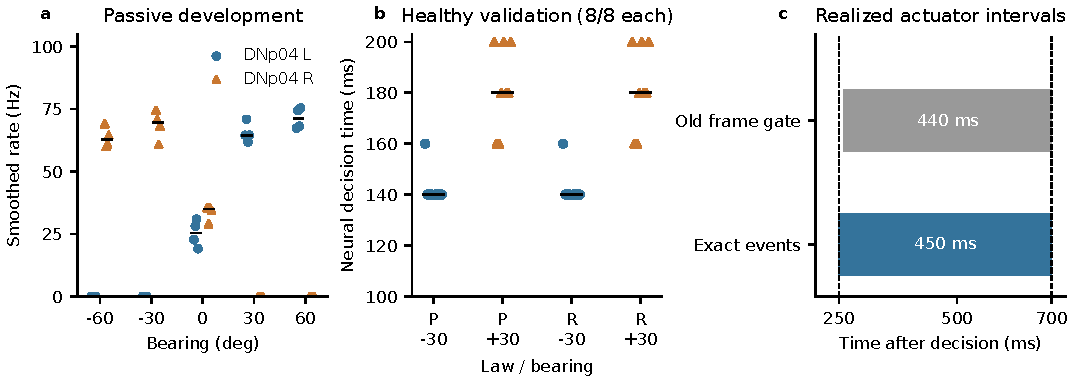
\includegraphics[width=\linewidth]{figs/development_v9.pdf}\caption{Development and validation diagnostics, not independent-test evidence. (a) DNp04 mean smoothed rates in 200--400 ms; all four developmental seeds per bearing, slight horizontal jitter for visibility, black median. (b) All eight validation seeds per law/bearing; P/R denote proportional/relay, black median. The same seed is shared across conditions. (c) Observed old completed bursts (four v8 records) and all 32 complete B-validation bursts, relative to decision time. This timing comparison does not isolate the cause of old-versus-new task outcomes; other controller/protocol components also changed.}\end{figure}

\section{Independent core outcomes and seed clusters}

\begin{table}[H]
\centering\small
\caption{Core outcomes. Each direction/law/dose has 24 seed clusters. L/G: healthy-to-fault losses/gains; H: healthy survivors at risk. Healthy rows compare to themselves.}
\begin{tabular}{lrrrrrr}
\toprule
Law & Network & $\phi$ & Success & L & G & H at risk\\
\midrule
proportional & healthy & -30 & 24/24 & 0 & 0 & 24\\
proportional & healthy & +30 & 24/24 & 0 & 0 & 24\\
proportional & F2\_25 & -30 & 23/24 & 1 & 0 & 24\\
proportional & F2\_25 & +30 & 23/24 & 1 & 0 & 24\\
proportional & F2\_50 & -30 & 14/24 & 10 & 0 & 24\\
proportional & F2\_50 & +30 & 23/24 & 1 & 0 & 24\\
relay & healthy & -30 & 24/24 & 0 & 0 & 24\\
relay & healthy & +30 & 24/24 & 0 & 0 & 24\\
relay & F2\_25 & -30 & 24/24 & 0 & 0 & 24\\
relay & F2\_25 & +30 & 24/24 & 0 & 0 & 24\\
relay & F2\_50 & -30 & 24/24 & 0 & 0 & 24\\
relay & F2\_50 & +30 & 24/24 & 0 & 0 & 24\\
\bottomrule
\end{tabular}
\end{table}

{\small
\begin{longtable}{lrrrrrrr}
\caption{Every core task outcome, 1=collision-free through 1000 ms. P/R: proportional/relay. H/25/50: healthy and row deletion percentages. No direction or failed seed is omitted.}\\
\toprule
Seed & $\phi$ & P H & P 25 & P 50 & R H & R 25 & R 50\\
\midrule\endfirsthead
\toprule
Seed & $\phi$ & P H & P 25 & P 50 & R H & R 25 & R 50\\
\midrule\endhead
1000 & -30 & 1 & 1 & 1 & 1 & 1 & 1\\
1000 & +30 & 1 & 1 & 1 & 1 & 1 & 1\\
1001 & -30 & 1 & 1 & 1 & 1 & 1 & 1\\
1001 & +30 & 1 & 1 & 1 & 1 & 1 & 1\\
1002 & -30 & 1 & 1 & 0 & 1 & 1 & 1\\
1002 & +30 & 1 & 1 & 1 & 1 & 1 & 1\\
1003 & -30 & 1 & 1 & 0 & 1 & 1 & 1\\
1003 & +30 & 1 & 1 & 1 & 1 & 1 & 1\\
1004 & -30 & 1 & 1 & 1 & 1 & 1 & 1\\
1004 & +30 & 1 & 1 & 1 & 1 & 1 & 1\\
1005 & -30 & 1 & 1 & 0 & 1 & 1 & 1\\
1005 & +30 & 1 & 0 & 1 & 1 & 1 & 1\\
1006 & -30 & 1 & 1 & 1 & 1 & 1 & 1\\
1006 & +30 & 1 & 1 & 0 & 1 & 1 & 1\\
1007 & -30 & 1 & 0 & 1 & 1 & 1 & 1\\
1007 & +30 & 1 & 1 & 1 & 1 & 1 & 1\\
1008 & -30 & 1 & 1 & 0 & 1 & 1 & 1\\
1008 & +30 & 1 & 1 & 1 & 1 & 1 & 1\\
1009 & -30 & 1 & 1 & 1 & 1 & 1 & 1\\
1009 & +30 & 1 & 1 & 1 & 1 & 1 & 1\\
1010 & -30 & 1 & 1 & 0 & 1 & 1 & 1\\
1010 & +30 & 1 & 1 & 1 & 1 & 1 & 1\\
1011 & -30 & 1 & 1 & 0 & 1 & 1 & 1\\
1011 & +30 & 1 & 1 & 1 & 1 & 1 & 1\\
1012 & -30 & 1 & 1 & 0 & 1 & 1 & 1\\
1012 & +30 & 1 & 1 & 1 & 1 & 1 & 1\\
1013 & -30 & 1 & 1 & 1 & 1 & 1 & 1\\
1013 & +30 & 1 & 1 & 1 & 1 & 1 & 1\\
1014 & -30 & 1 & 1 & 1 & 1 & 1 & 1\\
1014 & +30 & 1 & 1 & 1 & 1 & 1 & 1\\
1015 & -30 & 1 & 1 & 1 & 1 & 1 & 1\\
1015 & +30 & 1 & 1 & 1 & 1 & 1 & 1\\
1016 & -30 & 1 & 1 & 1 & 1 & 1 & 1\\
1016 & +30 & 1 & 1 & 1 & 1 & 1 & 1\\
1017 & -30 & 1 & 1 & 0 & 1 & 1 & 1\\
1017 & +30 & 1 & 1 & 1 & 1 & 1 & 1\\
1018 & -30 & 1 & 1 & 1 & 1 & 1 & 1\\
1018 & +30 & 1 & 1 & 1 & 1 & 1 & 1\\
1019 & -30 & 1 & 1 & 1 & 1 & 1 & 1\\
1019 & +30 & 1 & 1 & 1 & 1 & 1 & 1\\
1020 & -30 & 1 & 1 & 0 & 1 & 1 & 1\\
1020 & +30 & 1 & 1 & 1 & 1 & 1 & 1\\
1021 & -30 & 1 & 1 & 1 & 1 & 1 & 1\\
1021 & +30 & 1 & 1 & 1 & 1 & 1 & 1\\
1022 & -30 & 1 & 1 & 0 & 1 & 1 & 1\\
1022 & +30 & 1 & 1 & 1 & 1 & 1 & 1\\
1023 & -30 & 1 & 1 & 1 & 1 & 1 & 1\\
1023 & +30 & 1 & 1 & 1 & 1 & 1 & 1\\
\bottomrule
\end{longtable}
}

\begin{table}[H]
\centering\small
\caption{Complete-seed effects in percentage points; 20,000 percentile bootstrap resamples, seed 20261022, conditional on this model/map/task.}
\begin{tabular}{lrr}
\toprule
Seed-level estimand & Mean (pp) & 95\% interval (pp)\\
\midrule
proportional\_F2\_25\_net\_loss & 4.2 & [0.0, 10.4]\\
proportional\_F2\_50\_net\_loss & 22.9 & [12.5, 33.3]\\
relay\_F2\_25\_net\_loss & 0.0 & [0.0, 0.0]\\
relay\_F2\_50\_net\_loss & 0.0 & [0.0, 0.0]\\
F2\_25\_interaction & -4.2 & [-10.4, 0.0]\\
F2\_50\_interaction & -22.9 & [-33.3, -12.5]\\
\bottomrule
\end{tabular}
\end{table}

{\small
\begin{longtable}{lrrrrrr}
\caption{Every actual independent cluster contrast. P/R and 25/50 match the preceding table; interaction is R minus P net loss.}\\
\toprule
Seed & P25 & R25 & $\Delta25$ & P50 & R50 & $\Delta50$\\
\midrule\endfirsthead
\toprule
Seed & P25 & R25 & $\Delta25$ & P50 & R50 & $\Delta50$\\
\midrule\endhead
1000 & 0.00 & 0.00 & 0.00 & 0.00 & 0.00 & 0.00\\
1001 & 0.00 & 0.00 & 0.00 & 0.00 & 0.00 & 0.00\\
1002 & 0.00 & 0.00 & 0.00 & 0.50 & 0.00 & -0.50\\
1003 & 0.00 & 0.00 & 0.00 & 0.50 & 0.00 & -0.50\\
1004 & 0.00 & 0.00 & 0.00 & 0.00 & 0.00 & 0.00\\
1005 & 0.50 & 0.00 & -0.50 & 0.50 & 0.00 & -0.50\\
1006 & 0.00 & 0.00 & 0.00 & 0.50 & 0.00 & -0.50\\
1007 & 0.50 & 0.00 & -0.50 & 0.00 & 0.00 & 0.00\\
1008 & 0.00 & 0.00 & 0.00 & 0.50 & 0.00 & -0.50\\
1009 & 0.00 & 0.00 & 0.00 & 0.00 & 0.00 & 0.00\\
1010 & 0.00 & 0.00 & 0.00 & 0.50 & 0.00 & -0.50\\
1011 & 0.00 & 0.00 & 0.00 & 0.50 & 0.00 & -0.50\\
1012 & 0.00 & 0.00 & 0.00 & 0.50 & 0.00 & -0.50\\
1013 & 0.00 & 0.00 & 0.00 & 0.00 & 0.00 & 0.00\\
1014 & 0.00 & 0.00 & 0.00 & 0.00 & 0.00 & 0.00\\
1015 & 0.00 & 0.00 & 0.00 & 0.00 & 0.00 & 0.00\\
1016 & 0.00 & 0.00 & 0.00 & 0.00 & 0.00 & 0.00\\
1017 & 0.00 & 0.00 & 0.00 & 0.50 & 0.00 & -0.50\\
1018 & 0.00 & 0.00 & 0.00 & 0.00 & 0.00 & 0.00\\
1019 & 0.00 & 0.00 & 0.00 & 0.00 & 0.00 & 0.00\\
1020 & 0.00 & 0.00 & 0.00 & 0.50 & 0.00 & -0.50\\
1021 & 0.00 & 0.00 & 0.00 & 0.00 & 0.00 & 0.00\\
1022 & 0.00 & 0.00 & 0.00 & 0.50 & 0.00 & -0.50\\
1023 & 0.00 & 0.00 & 0.00 & 0.00 & 0.00 & 0.00\\
\bottomrule
\end{longtable}
}

\begin{table}[H]
\centering\small
\caption{Prespecified symmetric-null sign-flip sensitivity; not a randomized-controller assignment test.}
\begin{tabular}{lrr}
\toprule
Dose & Raw p & Holm p\\
\midrule
F2\_25 & 0.500000 & 0.500000\\
F2\_50 & 0.000977 & 0.001953\\
\bottomrule
\end{tabular}
\end{table}

The originally frozen analyzer passed the complete input/source/timing checks but then failed on duplicate numeric-margin/Boolean-warning CSV keys, before reporting statistics. The original script, failure log and output directory are retained. The documented exportfix analyzer renames only numeric CSV fields, preserving all numerical definitions, thresholds, source guards and raw records; canonical analyses are core-v2 and stress-v2. This is a post-registration analytical export correction, not a new hypothesis or neural rerun. See \path{paper/PROTOCOL_v9_NOTES.md}.

A post-hoc control diagnostic verifies identical first trigger times and pre-decision traces in all 144 paired law/scenario cells. Both laws gate steering below the trigger threshold, so their first action divergence follows that same decision. Table entries at 400 ms precede every contact. Equal maximum turn rate does not match executed turning effort; these diagnostics are not causal mediation estimates or energy measurements.

\begin{table}[H]
\centering\small
\caption{Descriptive precontact control diagnostics on all core records; medians pool the two paired directions, without adding independent samples.}
\begin{tabular}{lrrr}
\toprule
Law & Network & Median trigger (ms) & Median $|\theta(400)|$ (deg)\\
\midrule
proportional & healthy & 160.0 & 88.27\\
proportional & F2\_25 & 180.0 & 71.62\\
proportional & F2\_50 & 220.0 & 38.73\\
relay & healthy & 160.0 & 100.00\\
relay & F2\_25 & 180.0 & 100.00\\
relay & F2\_50 & 220.0 & 96.00\\
\bottomrule
\end{tabular}
\end{table}

\begin{table}[H]
\centering\small
\caption{Healthy baseline safety reserve over the full 1-s episode. No healthy record collided, so these values contain no post-contact continuation. Matching binary success does not match clearance or executed effort.}
\begin{tabular}{lrrrr}
\toprule
Law & Episodes & Median clearance (mm) & Minimum (mm) & Maximum (mm)\\
\midrule
proportional & 48 & 33.08 & 13.88 & 39.64\\
relay & 48 & 41.43 & 39.24 & 42.19\\
\bottomrule
\end{tabular}
\end{table}

\section{Frozen warnings, information and error denominators}

\begin{table}[H]
\centering\small
\caption{Thresholds learned only from all 32 healthy validation records.}
\begin{tabular}{lr}
\toprule
Criterion & Threshold\\
\midrule
Command mean, 100--400 ms & 5.833333333 Hz\\
Two-sided activity log score & 0.169456319\\
Held-command clearance & 0.018772702 m\\
Schedule-only clearance & 0.018548260 m\\
Upper resource excursion & $2\times$ reference\\
\bottomrule
\end{tabular}
\end{table}

All prospective warnings use data through 400 ms, verified before first contact in every record. The two-sided activity score is the absolute log count ratio to the law/side-specific validation median. Its cutoff is the healthy 95th percentile; command and forecast cutoffs are fifth percentiles. The same nominal 5\% healthy flag calibration is not a guarantee of task FPR. Held-command and schedule forecasts share exact simulated geometry and the pending actuator schedule; the candidate holds the current neural-derived turn command, the baseline sets future turn to zero. If no trigger exists, both assume the earliest next-frame decision. This is an optimistic extrapolation, not a neural-only detector or reachability proof.

{\small
\begin{longtable}{lrrrrrrrrr}
\caption{Core confusion counts. Positives are collisions through 1 s. The own-stop upper criterion is retrospective resource scoring, not a 400-ms warning. All/faulty/healthy subsets are overlapping views of the same seed clusters. A dash means the conditional rate is undefined because its class is absent.}\\
\toprule
Criterion & Subset & TP & FP & TN & FN & Sens & Spec & FPR & FNR\\
\midrule\endfirsthead
\toprule
Criterion & Subset & TP & FP & TN & FN & Sens & Spec & FPR & FNR\\
\midrule\endhead
Command low & all & 2 & 51 & 224 & 11 & 0.154 & 0.815 & 0.185 & 0.846\\
Command low & faulty & 2 & 49 & 130 & 11 & 0.154 & 0.726 & 0.274 & 0.846\\
Command low & healthy & 0 & 2 & 94 & 0 & -- & 0.979 & 0.021 & --\\
Own-stop upper & all & 3 & 8 & 267 & 10 & 0.231 & 0.971 & 0.029 & 0.769\\
Own-stop upper & faulty & 3 & 8 & 171 & 10 & 0.231 & 0.955 & 0.045 & 0.769\\
Own-stop upper & healthy & 0 & 0 & 96 & 0 & -- & 1.000 & 0.000 & --\\
400-ms upper & all & 0 & 0 & 275 & 13 & 0.000 & 1.000 & 0.000 & 1.000\\
400-ms upper & faulty & 0 & 0 & 179 & 13 & 0.000 & 1.000 & 0.000 & 1.000\\
400-ms upper & healthy & 0 & 0 & 96 & 0 & -- & 1.000 & 0.000 & --\\
Two-sided activity & all & 3 & 68 & 207 & 10 & 0.231 & 0.753 & 0.247 & 0.769\\
Two-sided activity & faulty & 3 & 54 & 125 & 10 & 0.231 & 0.698 & 0.302 & 0.769\\
Two-sided activity & healthy & 0 & 14 & 82 & 0 & -- & 0.854 & 0.146 & --\\
Actuator schedule & all & 13 & 84 & 191 & 0 & 1.000 & 0.695 & 0.305 & 0.000\\
Actuator schedule & faulty & 13 & 80 & 99 & 0 & 1.000 & 0.553 & 0.447 & 0.000\\
Actuator schedule & healthy & 0 & 4 & 92 & 0 & -- & 0.958 & 0.042 & --\\
Held-command candidate & all & 13 & 57 & 218 & 0 & 1.000 & 0.793 & 0.207 & 0.000\\
Held-command candidate & faulty & 13 & 55 & 124 & 0 & 1.000 & 0.693 & 0.307 & 0.000\\
Held-command candidate & healthy & 0 & 2 & 94 & 0 & -- & 0.979 & 0.021 & --\\
\bottomrule
\end{longtable}
}

The retrospective own-stop upper flag divides by its paired healthy stopped count. The prospective 400-ms activity flags instead use frozen law/side validation medians. Their classification difference therefore changes both observation and reference, and is not a pure exposure ablation. The duration-isolated comparison is $R_{\rm stop}$ versus $R_{\rm common}$ within the same healthy/fault pair. The two-sided score also detects low activity; it addresses a different hypothesis from an upper resource limit.

\begin{table}[H]
\centering\small
\caption{Secondary descriptive paired held-command minus schedule comparison (pp), added after registration. The same bootstrap draws keep complete seed clusters together. No extra confirmatory test or threshold tuning is introduced.}
\begin{tabular}{lrrr}
\toprule
Subset & Metric & Difference (pp) & 95\% interval (pp)\\
\midrule
all & sensitivity & 0.00 & [0.00, 0.00]\\
all & specificity & 9.82 & [6.57, 13.41]\\
all & error\_rate & -9.38 & [-12.85, -6.25]\\
faulty & sensitivity & 0.00 & [0.00, 0.00]\\
faulty & specificity & 13.97 & [9.44, 19.02]\\
faulty & error\_rate & -13.02 & [-17.71, -8.85]\\
healthy & sensitivity & -- & --\\
healthy & specificity & 2.08 & [0.00, 5.21]\\
healthy & error\_rate & -2.08 & [-5.21, 0.00]\\
\bottomrule
\end{tabular}
\end{table}

\begin{table}[H]
\centering\small
\caption{Sparse-class bootstrap diagnostics. A missing positive class makes sensitivity undefined; such draws are not silently treated as zero.}
\begin{tabular}{lrrrr}
\toprule
Subset & Positive clusters & Negative clusters & Valid sens. draws & Valid spec. draws\\
\midrule
all & 12 & 24 & 20000 & 20000\\
faulty & 12 & 24 & 20000 & 20000\\
healthy & 0 & 24 & 0 & 20000\\
\bottomrule
\end{tabular}
\end{table}

{\small
\begin{longtable}{lrrrrrrr}
\caption{Direction/law disaggregation of the same core warning records.}\\
\toprule
Criterion & Stratum & TP & FP & TN & FN & Sens & Spec\\
\midrule\endfirsthead
\toprule
Criterion & Stratum & TP & FP & TN & FN & Sens & Spec\\
\midrule\endhead
transmission & proportional/-30 & 1 & 0 & 61 & 10 & 0.091 & 1.000\\
transmission & proportional/30 & 1 & 12 & 58 & 1 & 0.500 & 0.829\\
transmission & relay/-30 & 0 & 13 & 59 & 0 & -- & 0.819\\
transmission & relay/30 & 0 & 26 & 46 & 0 & -- & 0.639\\
equal\_duration\_upper & proportional/-30 & 0 & 0 & 61 & 11 & 0.000 & 1.000\\
equal\_duration\_upper & proportional/30 & 0 & 0 & 70 & 2 & 0.000 & 1.000\\
equal\_duration\_upper & relay/-30 & 0 & 0 & 72 & 0 & -- & 1.000\\
equal\_duration\_upper & relay/30 & 0 & 0 & 72 & 0 & -- & 1.000\\
equal\_duration\_two\_sided & proportional/-30 & 2 & 12 & 49 & 9 & 0.182 & 0.803\\
equal\_duration\_two\_sided & proportional/30 & 1 & 8 & 62 & 1 & 0.500 & 0.886\\
equal\_duration\_two\_sided & relay/-30 & 0 & 25 & 47 & 0 & -- & 0.653\\
equal\_duration\_two\_sided & relay/30 & 0 & 23 & 49 & 0 & -- & 0.681\\
schedule\_only & proportional/-30 & 11 & 31 & 30 & 0 & 1.000 & 0.492\\
schedule\_only & proportional/30 & 2 & 37 & 33 & 0 & 1.000 & 0.471\\
schedule\_only & relay/-30 & 0 & 0 & 72 & 0 & -- & 1.000\\
schedule\_only & relay/30 & 0 & 16 & 56 & 0 & -- & 0.778\\
deadline & proportional/-30 & 11 & 27 & 34 & 0 & 1.000 & 0.557\\
deadline & proportional/30 & 2 & 21 & 49 & 0 & 1.000 & 0.700\\
deadline & relay/-30 & 0 & 0 & 72 & 0 & -- & 1.000\\
deadline & relay/30 & 0 & 9 & 63 & 0 & -- & 0.875\\
\bottomrule
\end{longtable}
}

Full conditional cluster intervals for sensitivity, specificity, FPR and FNR are in the source summary JSON. Resampling keeps every law/bearing/dose within seed together. Zero observed errors may produce a degenerate bootstrap interval; the one-sided 95\% bound for the probability of at least one error in an otherwise identically defined seed cluster is $1-0.05^{1/n}$. This is a cluster-any-error bound, not a conditional FPR/FNR guarantee. No population or hardware zero-risk claim follows.

The original registration gives an approximate 0.20 planning half-width without stating its range explicitly. This normal maximum-variance approximation applies only to $[0,1]$ success/loss/gain cluster means. Signed net loss spans $[-1,1]$, and its between-law contrast can span $[-2,2]$, yielding range-based planning approximations about 0.40 and 0.80, respectively. These are not finite-sample coverage guarantees. The clarification in \path{paper/PROTOCOL_v9_NOTES.md} preserves the registration bytes, sample size and analysis. Actual intervals are reported; small interactions and equivalence are not established by the sample size.

\section{Exposure and observation horizon}

{\small
\begin{longtable}{lrrr}
\caption{Paired network-spike estimands. Own-stop and common-duration use recorded first-contact frame ends. Fixed 1-s activity includes explicitly simulated post-contact continuation.}\\
\toprule
Law/dose & Estimand & Median & 95\% cluster interval\\
\midrule\endfirsthead
\toprule
Law/dose & Estimand & Median & 95\% cluster interval\\
\midrule\endhead
proportional/F2\_25 & stop\_ratio & 1.1018 & [1.0672, 1.2307]\\
proportional/F2\_25 & common\_ratio & 1.1018 & [1.0672, 1.2307]\\
proportional/F2\_25 & early\_ratio & 1.0311 & [1.0075, 1.0741]\\
proportional/F2\_25 & full\_ratio & 1.1018 & [1.0672, 1.2307]\\
proportional/F2\_50 & stop\_ratio & 1.5052 & [1.4078, 1.5928]\\
proportional/F2\_50 & common\_ratio & 1.5052 & [1.4078, 1.5935]\\
proportional/F2\_50 & early\_ratio & 0.9813 & [0.9286, 1.0276]\\
proportional/F2\_50 & full\_ratio & 1.5052 & [1.4078, 1.5962]\\
relay/F2\_25 & stop\_ratio & 1.0996 & [1.0331, 1.1568]\\
relay/F2\_25 & common\_ratio & 1.0996 & [1.0331, 1.1568]\\
relay/F2\_25 & early\_ratio & 1.0886 & [1.0197, 1.1406]\\
relay/F2\_25 & full\_ratio & 1.0996 & [1.0331, 1.1568]\\
relay/F2\_50 & stop\_ratio & 1.2567 & [1.1152, 1.3345]\\
relay/F2\_50 & common\_ratio & 1.2567 & [1.1152, 1.3345]\\
relay/F2\_50 & early\_ratio & 1.1844 & [1.0587, 1.2337]\\
relay/F2\_50 & full\_ratio & 1.2567 & [1.1152, 1.3345]\\
\bottomrule
\end{longtable}
}

\begin{table}[H]
\centering\small
\caption{Repeated fixed task horizons; these do not add independent samples. No endpoint was selected for significance.}
\begin{tabular}{lrrrr}
\toprule
Law & Network & 800 ms & 900 ms & 1000 ms\\
\midrule
proportional & healthy & 48/48 & 48/48 & 48/48\\
proportional & F2\_25 & 48/48 & 48/48 & 46/48\\
proportional & F2\_50 & 46/48 & 46/48 & 37/48\\
relay & healthy & 48/48 & 48/48 & 48/48\\
relay & F2\_25 & 48/48 & 48/48 & 48/48\\
relay & F2\_50 & 48/48 & 48/48 & 48/48\\
\bottomrule
\end{tabular}
\end{table}

Common duration is outcome-dependent and does not hold closed-loop sensory histories fixed. Full-horizon activity after first contact is a specified counterfactual resource measure, not a prospective predictor or a claim about physical contact dynamics. Activity profiles at 200/400/600/800/1000 ms, including counts of prior contacts at each window, are provided in activity-profiles.csv.

\begin{figure}[H]\centering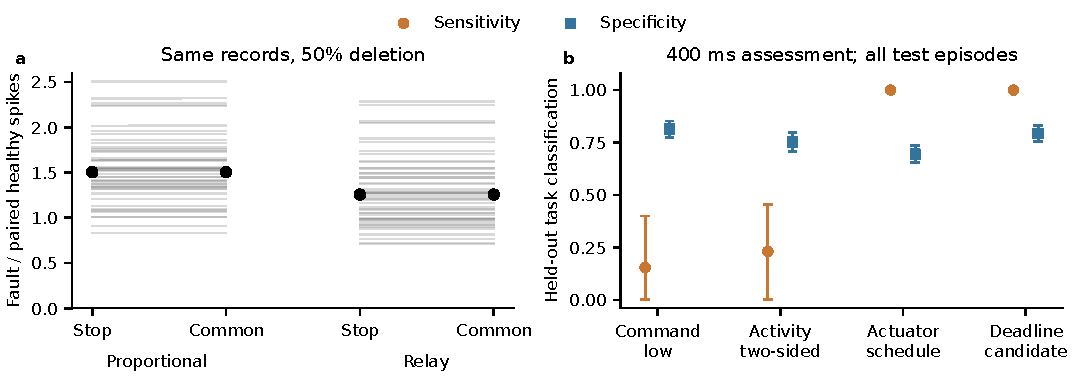
\includegraphics[width=\linewidth]{figs/task_v9_assessment.pdf}\caption{Core exposure estimands and frozen warning performance. Every line in the left panel is a matched scenario; black markers are medians. Right-panel intervals use complete seed-cluster resampling. The upper resource criterion and all subgroup errors remain tabulated even if they are not emphasized in the main figure.}\end{figure}

\section{Prespecified off-angle stress transfer}

The $\pm45^\circ$ test uses eight NEW seed clusters and unchanged laws, map, actuator and thresholds. These angles were absent from calibration and validation. The activity reference transfers from the same-side $30^\circ$ stratum. No threshold is fitted on stress outcomes, and stress records are not pooled with core records to strengthen inference. It tests angle transfer, not a new connectome or RF map. Eight-cluster uncertainty is necessarily wide.

\begin{table}[H]
\centering\small
\caption{Stress outcomes, eight clusters per law/direction/dose. Counts are separate from the 24-cluster core.}
\begin{tabular}{lrrrrrr}
\toprule
Law & Network & $\phi$ & Success & L & G & H at risk\\
\midrule
proportional & healthy & -45 & 8/8 & 0 & 0 & 8\\
proportional & healthy & +45 & 8/8 & 0 & 0 & 8\\
proportional & F2\_25 & -45 & 8/8 & 0 & 0 & 8\\
proportional & F2\_25 & +45 & 8/8 & 0 & 0 & 8\\
proportional & F2\_50 & -45 & 6/8 & 2 & 0 & 8\\
proportional & F2\_50 & +45 & 8/8 & 0 & 0 & 8\\
relay & healthy & -45 & 8/8 & 0 & 0 & 8\\
relay & healthy & +45 & 8/8 & 0 & 0 & 8\\
relay & F2\_25 & -45 & 8/8 & 0 & 0 & 8\\
relay & F2\_25 & +45 & 8/8 & 0 & 0 & 8\\
relay & F2\_50 & -45 & 8/8 & 0 & 0 & 8\\
relay & F2\_50 & +45 & 8/8 & 0 & 0 & 8\\
\bottomrule
\end{tabular}
\end{table}

{\small
\begin{longtable}{lrrrrrrr}
\caption{Every stress outcome. Definitions match the core outcome table.}\\
\toprule
Seed & $\phi$ & P H & P 25 & P 50 & R H & R 25 & R 50\\
\midrule\endfirsthead
\toprule
Seed & $\phi$ & P H & P 25 & P 50 & R H & R 25 & R 50\\
\midrule\endhead
1100 & -45 & 1 & 1 & 1 & 1 & 1 & 1\\
1100 & +45 & 1 & 1 & 1 & 1 & 1 & 1\\
1101 & -45 & 1 & 1 & 0 & 1 & 1 & 1\\
1101 & +45 & 1 & 1 & 1 & 1 & 1 & 1\\
1102 & -45 & 1 & 1 & 1 & 1 & 1 & 1\\
1102 & +45 & 1 & 1 & 1 & 1 & 1 & 1\\
1103 & -45 & 1 & 1 & 0 & 1 & 1 & 1\\
1103 & +45 & 1 & 1 & 1 & 1 & 1 & 1\\
1104 & -45 & 1 & 1 & 1 & 1 & 1 & 1\\
1104 & +45 & 1 & 1 & 1 & 1 & 1 & 1\\
1105 & -45 & 1 & 1 & 1 & 1 & 1 & 1\\
1105 & +45 & 1 & 1 & 1 & 1 & 1 & 1\\
1106 & -45 & 1 & 1 & 1 & 1 & 1 & 1\\
1106 & +45 & 1 & 1 & 1 & 1 & 1 & 1\\
1107 & -45 & 1 & 1 & 1 & 1 & 1 & 1\\
1107 & +45 & 1 & 1 & 1 & 1 & 1 & 1\\
\bottomrule
\end{longtable}
}

{\small
\begin{longtable}{lrrrrrrrrr}
\caption{Stress warning confusion counts; unchanged calibration and exact simulated geometry. Missing conditional rates remain undefined.}\\
\toprule
Criterion & Subset & TP & FP & TN & FN & Sens & Spec & FPR & FNR\\
\midrule\endfirsthead
\toprule
Criterion & Subset & TP & FP & TN & FN & Sens & Spec & FPR & FNR\\
\midrule\endhead
Command low & all & 1 & 40 & 54 & 1 & 0.500 & 0.574 & 0.426 & 0.500\\
Command low & faulty & 1 & 33 & 29 & 1 & 0.500 & 0.468 & 0.532 & 0.500\\
Command low & healthy & 0 & 7 & 25 & 0 & -- & 0.781 & 0.219 & --\\
Own-stop upper & all & 0 & 2 & 92 & 2 & 0.000 & 0.979 & 0.021 & 1.000\\
Own-stop upper & faulty & 0 & 2 & 60 & 2 & 0.000 & 0.968 & 0.032 & 1.000\\
Own-stop upper & healthy & 0 & 0 & 32 & 0 & -- & 1.000 & 0.000 & --\\
400-ms upper & all & 0 & 0 & 94 & 2 & 0.000 & 1.000 & 0.000 & 1.000\\
400-ms upper & faulty & 0 & 0 & 62 & 2 & 0.000 & 1.000 & 0.000 & 1.000\\
400-ms upper & healthy & 0 & 0 & 32 & 0 & -- & 1.000 & 0.000 & --\\
Two-sided activity & all & 0 & 43 & 51 & 2 & 0.000 & 0.543 & 0.457 & 1.000\\
Two-sided activity & faulty & 0 & 21 & 41 & 2 & 0.000 & 0.661 & 0.339 & 1.000\\
Two-sided activity & healthy & 0 & 22 & 10 & 0 & -- & 0.312 & 0.688 & --\\
Actuator schedule & all & 2 & 21 & 73 & 0 & 1.000 & 0.777 & 0.223 & 0.000\\
Actuator schedule & faulty & 2 & 21 & 41 & 0 & 1.000 & 0.661 & 0.339 & 0.000\\
Actuator schedule & healthy & 0 & 0 & 32 & 0 & -- & 1.000 & 0.000 & --\\
Held-command candidate & all & 2 & 11 & 83 & 0 & 1.000 & 0.883 & 0.117 & 0.000\\
Held-command candidate & faulty & 2 & 11 & 51 & 0 & 1.000 & 0.823 & 0.177 & 0.000\\
Held-command candidate & healthy & 0 & 0 & 32 & 0 & -- & 1.000 & 0.000 & --\\
\bottomrule
\end{longtable}
}

The stress set has only two failure clusters. Of 20000 bootstrap draws, 18024 contain a positive class and 1976 contain none. Reported sensitivity intervals condition on the valid draws; the zero observed miss interval is not a finite-sample guarantee. The joint new-cluster-any-miss upper bound is 31.2 percent, not a conditional FNR guarantee. The two-sided activity criterion also flags 22/32 healthy stress episodes: transferring the same-side 30-degree reference does not preserve its healthy flag calibration at 45 degrees.

\begin{table}[H]
\centering\small
\caption{Descriptive stress cluster effects, kept separate from the core analysis.}
\begin{tabular}{lrr}
\toprule
Seed-level estimand & Mean (pp) & 95\% interval (pp)\\
\midrule
proportional\_F2\_25\_net\_loss & 0.0 & [0.0, 0.0]\\
proportional\_F2\_50\_net\_loss & 12.5 & [0.0, 31.2]\\
relay\_F2\_25\_net\_loss & 0.0 & [0.0, 0.0]\\
relay\_F2\_50\_net\_loss & 0.0 & [0.0, 0.0]\\
F2\_25\_interaction & 0.0 & [0.0, 0.0]\\
F2\_50\_interaction & -12.5 & [-31.2, 0.0]\\
\bottomrule
\end{tabular}
\end{table}

\section{Separate motor-interface ablations}

Baseline walking remains 0.05 m/s when neural actions are disabled; the agent is not immobilized. Burst necessity follows from this toy plant by construction. For a walk-only segment of duration $\Delta t\leq0.02$ s with precontact separation $d\geq0.05$ m, the pursuer moves $0.3\Delta t$ toward the segment-start agent position and the agent moves at most $0.05\Delta t$. Since $d>0.3\Delta t$, triangle inequality gives $d_{\rm next}\leq d-(0.3-0.05)\Delta t$. From $d_0=0.25$ m, contact must occur by 0.8 s without a burst, regardless of heading commands. A lightweight geometry property test checks this bound over arbitrary commands. It is not an additional neural experiment or a newly fitted warning metric.

This diagnostic matrix was registered after the original core launch, before complete core analysis. It is not part of the original confirmatory registration and contributes no primary significance test. Eight new seeds 1200--1207 cross the two core bearings with normal proportional/relay, turn-disabled and steering-and-burst-disabled interfaces on healthy networks. The turn-disabled interface retains neural burst triggering; the other removes both neural actions. Common uniforms, calibration and physical settings remain fixed. Every normal failure and every ablated success is retained. The pair of ablations does not separately isolate burst necessity; the kinematic bound above establishes its necessity for this plant. These checks do not establish connectome-specific superiority or biological escape.

\begin{table}[H]
\centering\small
\caption{Independent diagnostic action outcomes. Each law/direction has eight clusters; this cohort is not pooled with core or stress.}
\begin{tabular}{lrrr}
\toprule
Interface & Bearing & Success & Triggered\\
\midrule
proportional & -30 & 8/8 & 8\\
proportional & +30 & 8/8 & 8\\
relay & -30 & 8/8 & 8\\
relay & +30 & 8/8 & 8\\
disabled & -30 & 0/8 & 8\\
disabled & +30 & 0/8 & 8\\
observe & -30 & 0/8 & 0\\
observe & +30 & 0/8 & 0\\
\bottomrule
\end{tabular}
\end{table}

{\small
\begin{longtable}{lrrrrr}
\caption{All action-ablation outcomes, 1=collision-free through 1 s. Turn off retains burst triggering; act off removes both actions.}\\
\toprule
Seed & Bearing & P & R & Turn off & Act off\\
\midrule\endfirsthead
\toprule
Seed & Bearing & P & R & Turn off & Act off\\
\midrule\endhead
1200 & -30 & 1 & 1 & 0 & 0\\
1200 & +30 & 1 & 1 & 0 & 0\\
1201 & -30 & 1 & 1 & 0 & 0\\
1201 & +30 & 1 & 1 & 0 & 0\\
1202 & -30 & 1 & 1 & 0 & 0\\
1202 & +30 & 1 & 1 & 0 & 0\\
1203 & -30 & 1 & 1 & 0 & 0\\
1203 & +30 & 1 & 1 & 0 & 0\\
1204 & -30 & 1 & 1 & 0 & 0\\
1204 & +30 & 1 & 1 & 0 & 0\\
1205 & -30 & 1 & 1 & 0 & 0\\
1205 & +30 & 1 & 1 & 0 & 0\\
1206 & -30 & 1 & 1 & 0 & 0\\
1206 & +30 & 1 & 1 & 0 & 0\\
1207 & -30 & 1 & 1 & 0 & 0\\
1207 & +30 & 1 & 1 & 0 & 0\\
\bottomrule
\end{longtable}
}

\begin{table}[H]
\centering\small
\caption{Descriptive normal-minus-ablated success differences (positive means normal succeeds more often), averaging bearings within each of eight clusters.}
\begin{tabular}{lrr}
\toprule
Seed-level estimand & Mean (pp) & 95\% interval (pp)\\
\midrule
proportional-minus-disabled & 100.0 & [100.0, 100.0]\\
proportional-minus-observe & 100.0 & [100.0, 100.0]\\
relay-minus-disabled & 100.0 & [100.0, 100.0]\\
relay-minus-observe & 100.0 & [100.0, 100.0]\\
\bottomrule
\end{tabular}
\end{table}

\section{Historical audit and preserved exploratory evidence}

These tables describe older protocols and are not independent v9 evidence. The v8 original/pre-cue-gated laws, global Brian2 input seeds and stop-on-collision semantics differ from v9. Its six clusters cannot be pooled with the new laws or called confirmed by a different controller comparison. The original 25\% interaction vector [0,0.5,0.5,0,0.5,0] has mean 0.25 and post-hoc symmetric-null p=0.25; the 50\% contrast is baseline-driven because both faulty laws have zero survivors. The conditional 25\% percentile interval [0.0833,0.4167] does not override the sparse support.

\begin{table}[H]
\centering\small
\caption{Preserved v8 counts independently reconstructed from its 72 records.}
\begin{tabular}{lrrrr}
\toprule
Law & Fault & -30 & +30 & Total\\
\midrule
brain & healthy & 4 & 0 & 4/12\\
brain & F2\_25 & 4 & 0 & 4/12\\
brain & F2\_50 & 0 & 0 & 0/12\\
precue\_gated & healthy & 6 & 0 & 6/12\\
precue\_gated & F2\_25 & 3 & 0 & 3/12\\
precue\_gated & F2\_50 & 0 & 0 & 0/12\\
\bottomrule
\end{tabular}
\end{table}

The source-qualified old-flag audit covers 96 unique records; 6 have an incorrect exact-horizon label. Reused copies are deduplicated. Another 57 old records lack sufficient exact generation-source/timing metadata for this audit; current code is not substituted for that missing provenance. Raw files remain unchanged.

\begin{table}[H]
\centering\small
\caption{Corrected derived v8 flags: all listed intervals end exactly at the 1-s horizon. Their last-frame state is true but exact-horizon state is false.}
\begin{tabular}{lrrrrr}
\toprule
Law & Fault & Seed & Bearing & Recorded & Exact\\
\midrule
brain & F2\_25 & 13 & -30 & 1 & 0\\
brain & F2\_25 & 15 & -30 & 1 & 0\\
brain & healthy & 15 & -30 & 1 & 0\\
brain & healthy & 17 & -30 & 1 & 0\\
precue\_gated & F2\_25 & 17 & -30 & 1 & 0\\
precue\_gated & healthy & 13 & -30 & 1 & 0\\
\bottomrule
\end{tabular}
\end{table}

Old nominal 250/450-ms actuation is realized as 260-ms delay and 440-ms completed bursts on 20-ms frame starts. Original/gated healthy survivors active at the exact horizon number two/two, versus four/three during the last frame. These metadata corrections do not change recorded survival. New v9 exact-event runs are separately executed and replay-checked; they do not retroactively validate old trajectories.

\begin{table}[H]
\centering\small
\caption{Read-only 600-ms archive recomputation. f is row deletion; p=1-f is survival. No universal power law or recruitment mechanism follows.}
\begin{tabular}{lrrr}
\toprule
f & p & Output retention & Retention/p\\
\midrule
0.05 & 0.95 & 0.9703 & 1.0214\\
0.10 & 0.90 & 0.9835 & 1.0928\\
0.25 & 0.75 & 0.8922 & 1.1896\\
0.50 & 0.50 & 0.7646 & 1.5292\\
\bottomrule
\end{tabular}
\end{table}

Historical transmission-only/joint scoring gives 276/288 versus 262/288 on the SAME records, not runs of SpikeFI or SpikingJET. The 14 differences are 12 inhibitory-hub and two random expected-contact-mass trials (zero-based trials 3 and 9: 327246 and 271058 spikes). Expected contact-mass matching does not equate row fractions (about 8.63\% versus 5.57\%). Their median does not remove the tail risk. HUB\_inh median/mean are 847476.5/847857 spikes. At 75-Hz drive, 50\% deletion passes the historical 51.4-Hz criterion in only 10/12 cases; the 150-Hz main result does not extend to all drives.

\begin{table}[H]
\centering\small
\caption{Preserved legacy closed-loop records. Bursts mean any logged burst interval, not exact-horizon activity. Geometry/calibration are compromised; this is a descriptive audit.}
\begin{tabular}{lrrrr}
\toprule
Cohort & Survival & Bursts & Above 2x & Median pair ratio\\
\midrule
v4/F4\_1pct & 12/12 & 12 & 6 & 1.7029\\
v4/F2\_25 & 10/12 & 10 & 0 & 0.8861\\
v4/F2\_50 & 0/12 & 0 & 0 & 0.3817\\
v4c/HUB\_inh & 6/12 & 12 & 12 & 71.6931\\
\bottomrule
\end{tabular}
\end{table}

F4 has 12/12 survival but 6/12 twofold activity exceedances; its pooled ratio near 1.7 is not a per-condition pass. Legacy 50\% deletion changes median ratio from 0.381701 to 0.729443 under common-duration matching. Original F4 node manifests remain unavailable; current reconstructed/protected-FlyID selectors cannot recover those identities or validate the original dynamics. Corrected hub causal experiments are not claimed. The v9 main test uses only row deletion and does not depend on those hub selections.

\section{Compute, audit scope and exact artifact access}

\begin{table}[H]
\centering\small
\caption{Measured episode wall times. Overlapping worker sums are NOT CPU seconds or campaign elapsed time.}
\begin{tabular}{lrrr}
\toprule
Cohort & Episodes & Median episode (s) & Episode sum (s)\\
\midrule
Core & 288 & 145.51 & 43040.80\\
Stress & 96 & 133.00 & 12600.25\\
Action ablation & 64 & 131.40 & 8401.72\\
\bottomrule
\end{tabular}
\end{table}

The exercised runtime is CPython 3.12.14, Brian2 2.10.1, NumPy 2.5.4, Cython 3.1.3 (NumPy code generation), on a Windows CPU host with 31.59 GiB physical memory. Full pins, source/input hashes and actual launcher elapsed/exit-code records accompany the artifact. No hardware mapping, energy, area, physical upset rate or real-time neural execution is inferred. The independent audit checks trace/input consistency using recorded readout outputs; it does not verify every neural state or replace full simulation.

The versioned source/data archive binds the main and supplementary PDFs to TeX, figures, CSV/JSON analysis, every independent raw episode, maps, registrations and exact generating snapshots. External connectivity/completeness tables and dependency caches are excluded; expected input hashes and the upstream release are specified. Reanalysis and input/geometry replay need no external table or new neural execution. Fresh simulation needs the external model and a Git checkout. The public repository may contain an earlier revision; a local archive is not public availability or evidence of submission. See \path{docs/REPRODUCE_v9.md} and the final material index. Historical source/timestep gaps remain explicit.

\end{document}